\documentclass{article}

\usepackage{microtype}
\usepackage{booktabs}
\usepackage{balance}
\usepackage{graphicx}
\usepackage{xcolor}
\usepackage{tikz}
\usetikzlibrary{arrows.meta,backgrounds,fit,positioning}
\usepackage{hyperref}
\newcommand{\theHalgorithm}{\arabic{algorithm}}
\usepackage[accepted]{icml2025}
\setcitestyle{numbers,square}

\definecolor{TUred}{RGB}{165,30,55}
\definecolor{TUdark}{RGB}{50,65,75}
\definecolor{TUblue}{RGB}{0,105,170}
\definecolor{TUgold}{RGB}{180,145,45}
\definecolor{TUgreen}{RGB}{80,135,80}
\hypersetup{
  colorlinks=true,
  hypertexnames=false,
  linkcolor=TUblue,
  citecolor=TUblue,
  urlcolor=TUblue
}

\setlength{\floatsep}{6pt}
\setlength{\textfloatsep}{7pt}
\setlength{\intextsep}{5pt}
\setlength{\abovecaptionskip}{3pt}
\setlength{\belowcaptionskip}{0pt}

\icmltitlerunning{Focused Hybrid Retrieval for Tübingen}

\begin{document}

\twocolumn[
\icmltitle{Focused Hybrid Retrieval for English Tübingen Web Content}

\begin{icmlauthorlist}
\icmlauthor{Julian Jurcevic}{equal}
\icmlauthor{Arne Hobrlant}{equal}
\icmlauthor{Andreas von Bendemann}{equal}
\end{icmlauthorlist}

\icmlaffiliation{equal}{University of Tübingen}
\icmlkeywords{focused crawling, information retrieval, hybrid search, search interface}
\vskip 0.15in
]

\begin{abstract}
We present an end-to-end search engine for English web content related to
Tübingen. The system combines a resumable focused crawler, a self-implemented
BM25F first stage, semantic second-stage re-ranking, batch retrieval, and an
interactive result interface. In a diagnostic 20-query ablation, semantic
re-ranking outperforms BM25F and the evaluated proximity bonus does not improve
effectiveness. After configuration was frozen, re-ranking improved nDCG@10
from 0.4867 to 0.5300 on a separate 10-query test set.
\end{abstract}

\section{Introduction}
The project requires a local search engine for English Tübingen-related web
content. It must cover crawling, indexing, retrieval of 100 results, batch
evaluation, and an interface that goes beyond a conventional ranked list. Our
system implements this complete pipeline and uses semantic re-ranking as its
retrieval innovation. This report describes the main design choices and uses a
controlled ablation to justify the final ranking configuration.

\section{System Overview}
The system separates offline collection and indexing from online retrieval.
The crawler stores accepted pages locally, after which the indexer constructs a
field-aware inverted index and document embeddings. At query time, BM25F
retrieves 100 candidates. A semantic model scores only these candidates, and
the fused ranking is returned through the API, batch command, and interactive
interface.

The \href{https://github.com/julilili42/search-engine}{search system}
(\texttt{SEARCH-COMMIT}) and
\href{https://github.com/julilili42/labeling-lab/tree/a81e4957cf8ebe00183c47a51650002ee6dc1386}{crawl-model training}
(\texttt{a81e495}) are maintained in separate repositories.

\section{Focused Crawling and Storage}
\subsection{Crawl Strategy}
Seeds were selected manually, favoring aggregator pages expected to expose
many relevant outgoing links. Sitemaps declared in \texttt{robots.txt} add up
to 1,000 same-origin URLs per seed origin to the frontier. The focused crawler
prioritizes links that are likely to lead to Tübingen-related content. It
follows the Robots Exclusion Protocol \citep{rfc9309} and filters fetched pages
using the HTML \texttt{lang} attribute. Multiple
workers consume a global priority frontier organized into per-host queues,
with at most one active request per host. Host cooldowns, page caps, and early
stopping after repeated rejects prevent individual domains from dominating the
collection.
Separately, Serper, a Google Search results API, was used to discover pages
for offline \textsc{PageVerdict} labeling \citep{serper}.

\subsection{Learned Focus Control}
Static URL and keyword heuristics proved too rigid in early qualitative
experiments. We therefore use a teacher--student setup to learn crawl-focus
signals from human judgments and Qwen-generated labels \citep{qwen25}. Limited
manual-labeling capacity motivated the use of LLM supervision \citep{wang2021}.
The resulting lightweight student models keep the collection compact while
favoring relevant, useful pages.

\textsc{PageVerdict} evaluates fetched pages, while \textsc{LinkVerdict}
prioritizes the links extracted from them. Both use word- and character-level
TF--IDF with class-balanced logistic regression. \textsc{PageVerdict} uses the
title, URL, metadata snippet, and visible page text. \textsc{LinkVerdict} uses
the anchor text, target and parent URLs, crawl depth, and the parent page's
\textsc{PageVerdict} signal. Data are split by destination host into disjoint
training, validation, and test sets. Five-fold grouped cross-validation selects
the regularization strength, and decision thresholds are selected on the
validation set.

Figure~\ref{fig:verdict-training} summarizes offline training, and
Figure~\ref{fig:crawler-runtime} shows the crawl loop. For
\textsc{PageVerdict}, Qwen~2.5:7B provides weak labels under a frozen
\href{https://github.com/julilili42/labeling-lab/blob/a81e4957cf8ebe00183c47a51650002ee6dc1386/src/auto_labeling/prompts/page-v4.txt}{prompt (\texttt{page-v4})},
alongside human judgments. German pages receive negative labels regardless of topical
relevance. However, the student model still accepts some pages with misleading
English metadata, \texttt{/en/} URLs, or English navigation around German main
content.
\textsc{LinkVerdict} uses human labels only because qualitative
inspection indicated that Qwen's judgments were less reliable with the limited
link context. Table~\ref{tab:verdict-benchmark}
reports performance on manually labeled test sets of 147 \textsc{PageVerdict}
and 546 \textsc{LinkVerdict} examples.

\begin{figure}[t]
  \centering
  \resizebox{\columnwidth}{!}{%
  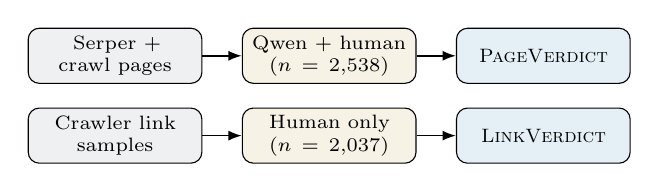
\begin{tikzpicture}[
    baseline=(current bounding box.south),
    node distance=3mm and 5mm,
    box/.style={
      draw,
      rounded corners,
      align=center,
      font=\scriptsize,
      minimum height=7mm,
      text width=21mm,
      inner sep=1.5pt
    },
    arrow/.style={-{Latex[length=1.7mm]}, semithick}
  ]
    \node[box, fill=TUdark!8] (page-samples) {Serper +\\crawl pages};
    \node[box, fill=TUgold!12, right=of page-samples] (page-labels)
      {Qwen + human\\($n=2{,}538$)};
    \node[box, fill=TUblue!10, right=of page-labels] (page-model)
      {\textsc{PageVerdict}};

    \node[box, fill=TUdark!8, below=of page-samples] (link-samples)
      {Crawler link\\samples};
    \node[box, fill=TUgold!12, right=of link-samples] (link-labels)
      {Human only\\($n=2{,}037$)};
    \node[box, fill=TUblue!10, right=of link-labels] (link-model)
      {\textsc{LinkVerdict}};

    \draw[arrow] (page-samples) -- (page-labels);
    \draw[arrow] (page-labels) -- (page-model);
    \draw[arrow] (link-samples) -- (link-labels);
    \draw[arrow] (link-labels) -- (link-model);
  \end{tikzpicture}
  }
  \caption{Offline training of the TF--IDF logistic-regression verdict models.}
  \label{fig:verdict-training}
\end{figure}

\begin{figure}[t]
  \centering
  \resizebox{\columnwidth}{!}{%
  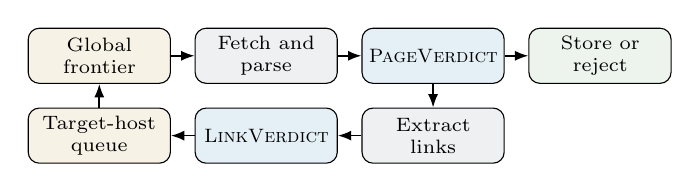
\begin{tikzpicture}[
    baseline=(current bounding box.south),
    node distance=3mm,
    box/.style={
      draw,
      rounded corners,
      align=center,
      font=\scriptsize,
      minimum height=7mm,
      text width=17mm,
      inner sep=1.5pt
    },
    arrow/.style={-{Latex[length=1.7mm]}, semithick}
  ]
    \node[box, fill=TUgold!12] (frontier) {Global\\frontier};
    \node[box, fill=TUdark!8, right=of frontier] (fetch) {Fetch and\\parse};
    \node[box, fill=TUblue!10, right=of fetch] (page)
      {\textsc{PageVerdict}};
    \node[box, fill=TUgreen!10, right=of page] (decision)
      {Store or\\reject};

    \node[box, fill=TUgold!12, below=of frontier] (queue)
      {Target-host\\queue};
    \node[box, fill=TUblue!10, below=of fetch] (link)
      {\textsc{LinkVerdict}};
    \node[box, fill=TUdark!8, below=of page] (extract)
      {Extract\\links};

    \draw[arrow] (frontier) -- (fetch);
    \draw[arrow] (fetch) -- (page);
    \draw[arrow] (page) -- (decision);
    \draw[arrow] (page) -- (extract);
    \draw[arrow] (extract) -- (link);
    \draw[arrow] (link) -- (queue);
    \draw[arrow] (queue) -- (frontier);
  \end{tikzpicture}
  }
  \caption{Runtime crawl loop. \textsc{LinkVerdict} scores extracted links
  before admission to the target host queue.}
  \label{fig:crawler-runtime}
\end{figure}

\subsection{Persistence and Collection Statistics}
URLs are normalized and deduplicated before entering the frontier. After
fetching, a 64-bit SimHash over token trigrams rejects fingerprints within a
Hamming distance of three from an accepted page \citep{manku2007}.
Accepted HTML is stored locally, while crawl metadata and model decisions are
persisted in SQLite. The frontier and deduplication state can be restored after
interruption.

\begin{table}[t]
  \centering
  \caption{Final crawl statistics. Hosts are domains represented in the
  accepted collection. Duplicates are a subset of rejected pages.}
  \label{tab:crawl-statistics}
  \small
  \setlength{\tabcolsep}{3.5pt}
  \begin{tabular}{@{}rrrrr@{}}
    \toprule
    Fetched & Accepted & Rejected & Duplicates & Hosts \\
    \midrule
    23,943 & 10,028 & 13,915 & 2,425 & 325 \\
    \bottomrule
  \end{tabular}
\end{table}

The final crawl fetched 23,943 pages, of which 10,028 (41.9\%) were accepted.

\begin{table}[t]
  \centering
  \caption{Performance on human-labeled test sets. Q and H denote
  Qwen~2.5:7B and human training labels, respectively.}
  \label{tab:verdict-benchmark}
  \small
  \setlength{\tabcolsep}{3pt}
  \begin{tabular}{@{}lrrrrr@{}}
    \toprule
    Model & $n$ & Bal.\ Acc. & F1 & ROC--AUC & AP \\
    \midrule
    Page (Q+H) & 147 & 0.692 & 0.709 & 0.774 & 0.720 \\
    Page (H) & 147 & 0.624 & 0.599 & 0.719 & 0.730 \\
    Link (H) & 546 & 0.746 & 0.629 & 0.822 & 0.627 \\
    \bottomrule
  \end{tabular}
\end{table}

\section{Indexing and Ranking}

\subsection{Language Safeguard}
An offline Lingua audit \citep{lingua} found that 24.9\% of accepted pages had
at least half of their classified German/English words assigned to German.
Indexing therefore checks the extracted main content independently. In
Lingua's low-accuracy mode for long text, pages with at least 20 classified
words are excluded when at least 80\% are assigned to languages other than
English. This conservative safeguard excluded 1,433 pages, reducing the final
index from 10,028 to 8,595 documents without altering the stored crawl.

\subsection{Lexical Retrieval}
After Unicode normalization, text is lowercased, split into alphanumeric
tokens, and filtered for single-character tokens and English stopwords. The
Rust-backed \texttt{py-rust-stemmers} package applies English Snowball stemming
to all index fields and queries \citep{pyruststemmers}; unstemmed body tokens
remain for snippets. Stemmed body positions support proximity scoring. The
index is serialized with MessagePack. On the
complete 8,595-document index, MessagePack was 37\% smaller than compact JSON
(44.1 vs.\ 70.0\,MB), while compact JSON took 2.84 times as long to
deserialize over 20 runs (624 vs.\ 220\,ms). For term $t$, document $d$, and fields $f$,
BM25F computes
\[
\tilde f_{t,d}=\sum_f w_f
\frac{f_{t,d,f}}{1-b+b\,|d_f|/\overline{|d_f|}},
\]
\[
s_{\mathrm{BM25F}}(d,q)=
\sum_{t\in q}\mathrm{IDF}(t)\frac{\tilde f_{t,d}}{k_1+\tilde f_{t,d}}.
\]
We use $b=0.75$ and $k_1=1.2$, preventing repeated term occurrences from
dominating the score \citep{robertson2004bm25f}. Based on qualitative experiments,
the body, title, and URL weights are 1, 5, and 3, respectively.

We also evaluated a lightly weighted proximity signal inspired by prior
extensions of Okapi scoring \citep{rasolofo2003}, but disabled it because it did
not improve retrieval quality.

\subsection{Semantic Retrieval and Fusion}
The second stage uses the general-purpose
\texttt{nli-mpnet-base-v2} encoder, whose sentence-embedding training uses
SNLI and MultiNLI natural-language-inference data
\citep{nli-mpnet-base-v2}. To prevent relevant content from being diluted on
long pages, documents are split into up to 20 overlapping 2,000-character
passages, with titles embedded separately. With cosine
similarity between the query $q$, title $t_d$, and passages $p_i$, the
heuristically weighted semantic score is
\[
\begin{array}{rl}
s_{\mathrm{sem}}(d,q)={}&0.20\cos(q,t_d)\\
&+0.65\max_i\cos(q,p_i)\\
&+0.15\,\mathrm{mean}_{i\in\mathrm{top3}}\cos(q,p_i).
\end{array}
\]
Semantic evidence is computed only for the 100 BM25F candidates. The final
score is
\[
s_{\mathrm{final}}(d,q)=\alpha\,\hat{s}_{\mathrm{BM25F}}(d,q)
  +\beta\,\hat{s}_{\mathrm{sem}}(d,q),
\]
where $\hat{s}_{\mathrm{BM25F}},\hat{s}_{\mathrm{sem}}\in[0,1]$ are obtained
by independently min--max normalizing both candidate score vectors. With
non-negative $\alpha+\beta=1$, $s_{\mathrm{final}}\in[0,1]$. We tested mixture
weights in increments of 0.1 on the development queries and selected
$\alpha=0.4$ and $\beta=0.6$ because they achieved the highest nDCG@10. A
repeat of the sweep after the final language safeguard and stemming selected
the same weights.
Missing or incompatible embeddings fall back to BM25F.

\section{Evaluation}
We first use 20 development queries covering broad topics, named entities, and
specific tasks to select the retrieval design. The pool unites the top 20 from
the four ablation variants, all eleven fusion weights, and the corresponding
no-stemming baseline. A single assessor grades each query--URL pair from 0
(irrelevant) to 3 (highly relevant) using URL, title, and snippet. We select
the design and
$\alpha/\beta$ by nDCG@10, then freeze them. Before retrieval, we define ten
new test queries covering distinct local and informational needs absent from
development. After the final language safeguard and stemming were applied, we
reran the frozen variants, repeated the weight sweep, and judged newly surfaced
pooled results. The repeated sweep confirmed rather than changed the frozen
weights. The test pool contains 530 judgments and the development pool 1,209. nDCG@20,
MRR@10, and warmed API latency provide complementary evidence.
Latency includes query encoding in a warmed process, but excludes startup,
artifact loading, HTTP transport, and rendering.

\begin{table*}[t]
\centering
\caption{Development ablation and frozen test results. Semantic scoring
re-ranks BM25F's top 100. Latency is mean warmed API time.}
\label{tab:retrieval-evaluation}
\small
\setlength{\tabcolsep}{6pt}
\begin{tabular}{@{}llccrrrr@{}}
\toprule
Set & Variant & Proximity & Semantic & nDCG@10 & nDCG@20 & MRR@10 & ms/query \\
\midrule
Dev. (20) & BM25F    & no  & no  & 0.5434 & 0.5394 & 0.9250 &  2.01 \\
 & BM25F + proximity & yes & no  & 0.5310 & 0.5308 & 0.9167 & 15.30 \\
 & BM25F + semantic  & no  & yes & \textbf{0.6260} & \textbf{0.6252} &
  \textbf{0.9375} & 56.12 \\
 & Full              & yes & yes & 0.6061 & 0.6191 & 0.9333 & 59.33 \\
\midrule
Test (10) & BM25F    & no  & no  & 0.4867 & 0.5002 & 0.8250 & 2.10 \\
 & BM25F + semantic  & no  & yes & \textbf{0.5300} & \textbf{0.5989} &
  \textbf{0.8500} & 79.40 \\
\bottomrule
\end{tabular}
\end{table*}

Semantic re-ranking improves development nDCG@10 by 0.0826 over BM25F, whereas proximity
reduces effectiveness both alone and in the full system. We therefore select
BM25F with semantic re-ranking and $\alpha=0.4,\beta=0.6$.
Table~\ref{tab:retrieval-evaluation} also reports the subsequent frozen test
evaluation.

\section{Result Presentation}
The presentation aims to expose retrieved URLs in a more creative form than a
conventional result list. Inspired by the Internet as a network of
interconnected networks, the interface maps results to stellar constellations
through which the user can navigate as a galaxy. The web client presents ten
clickable result cards alongside ten result stars
(Figure~\ref{fig:interface}). Star size and color encode the result-set
min--max-normalized final score, while vertical position follows rank by
default. Users may define semantic \(x\)- and \(y\)-axes through category
labels, onto which the server projects centered and bounded document
embeddings. In Figure~\ref{fig:interface}(b), \emph{river} and \emph{city}
organize this projection, separating results about the Neckar river from
geographic entities such as Neckar-Alb. Overlapping stars fan out on hover,
and pagination pans the camera between result constellations. The spatial view
augments the ranked cards without altering retrieval order.
The web client supports batch retrieval through TSV query uploads and
downloadable TSV results.

\begin{figure*}[t]
  \centering
  \begin{minipage}[t]{.36\textwidth}
    \centering
    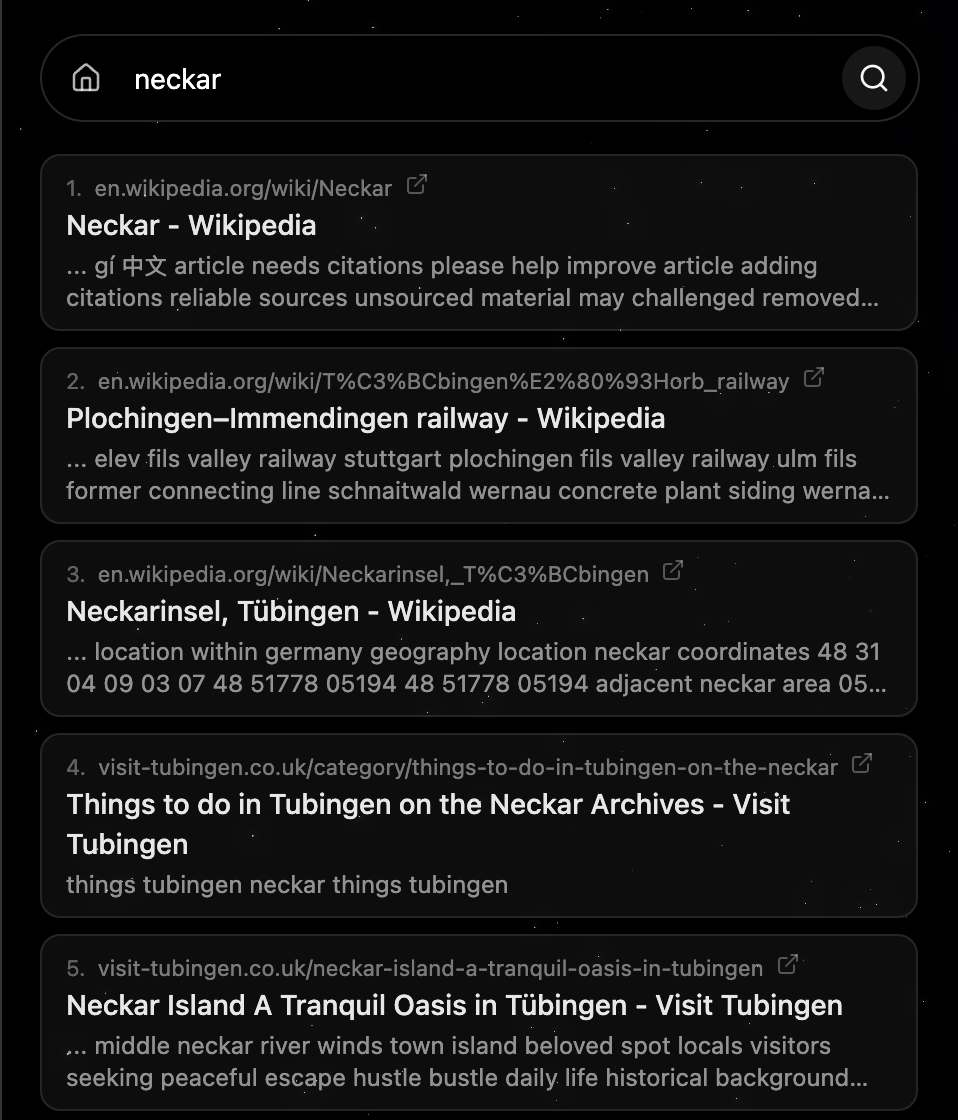
\includegraphics[height=.30\textheight]{img/result_list.png}\\[-1mm]
    {\scriptsize (a) Ranked result list.}
  \end{minipage}\hfill
  \begin{minipage}[t]{.62\textwidth}
    \centering
    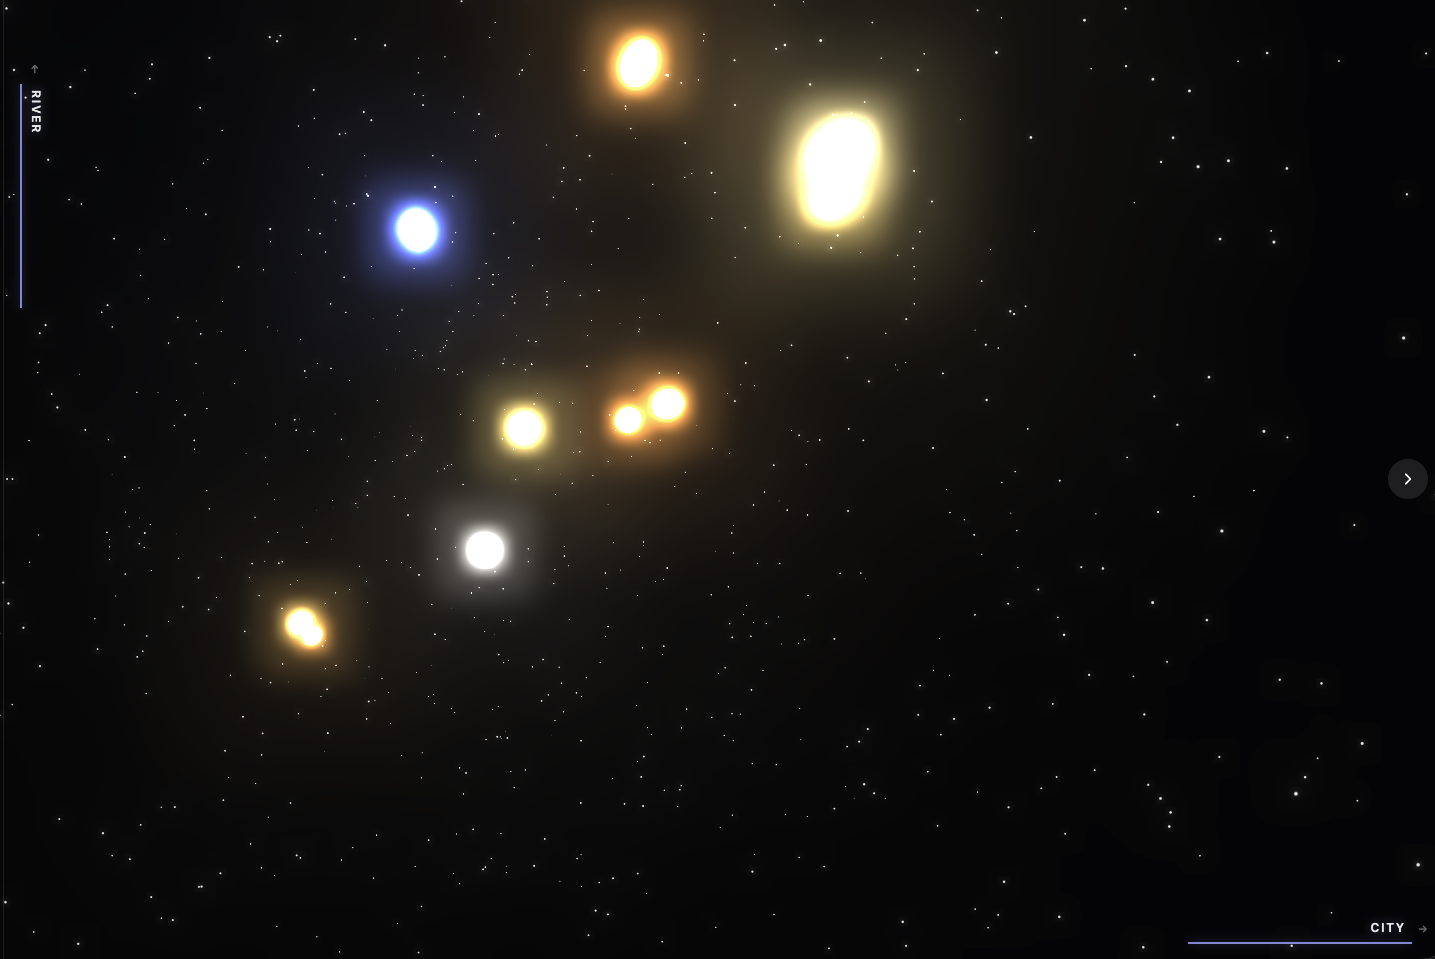
\includegraphics[height=.30\textheight]{img/star_constellation.png}\\[-1mm]
    {\scriptsize (b) Category-based star constellation.}
  \end{minipage}
  \caption{Implemented search interface with ranked cards and a semantic
  constellation.}
  \label{fig:interface}
\end{figure*}

\section{Limitations}
Collection coverage is source-skewed: 45.0\% of accepted pages come from the
University of Tübingen and its subdomains. Future work could improve source
diversity through organization-level crawl budgets and stronger saturation
penalties.

A single assessor limits the robustness of the relevance judgments. Moreover,
ten queries are insufficient to establish statistical significance or
superiority beyond this collection.

The verdict benchmarks use one labeling policy and relatively small test sets,
including the 147-example \textsc{PageVerdict} comparison set. Their results
therefore support the crawler design but do not establish performance on other
domains.

\balance
\section{Conclusion}
The implemented system covers the path from focused crawling to batch and
interactive retrieval. The development ablation selects semantic re-ranking of
BM25F candidates, and the separate test improves all three reported metrics
on these queries. The official pooled course evaluation will provide the final
external measure of effectiveness.

\bibliography{bibliography}
\bibliographystyle{unsrtnat}

\end{document}
